\documentclass{article}

% Packages
\usepackage{amsmath, amsfonts, amssymb, amsthm, bm, bbm, comment} 
\usepackage{enumerate, graphicx, xcolor, tcolorbox, hyphenat, circledsteps}
\usepackage[shortlabels]{enumitem}
\usepackage{url, hyperref}
\hypersetup{
	colorlinks   = true,
	urlcolor     = cyan,
	linkcolor    = red,
	citecolor    = black
}

% Formatting
\usepackage[a4paper, noheadfoot, scale={0.7,0.8}]{geometry}
\title{Wk 5 Supervision Problems 2}
\author{Luca Bollini}
\date{05 November 2026}
\hyphenpenalty=10000

% Commands
\newcommand{\N}{\mathbb{N}}
\newcommand{\Z}{\mathbb{Z}}
\newcommand{\Q}{\mathbb{Q}}
\newcommand{\R}{\mathbb{R}}
\newcommand{\eps}{\varepsilon}
\newcommand{\ddt}[1]{\frac{d}{d#1}}
\newcommand{\ddttwo}[1]{\frac{d^2}{d#1^2}}
\newcommand{\ts}{\thinspace}

% Colours
\newtcolorbox{questionbox}{
	colframe=black, 
	colback=white, 
	boxrule=0.2mm,
	arc=0mm,
}

\begin{document}
\maketitle

\begin{comment}
    NOTE!
    This week is a bit lighter as I plan on revisiting some of the previous worksheets with problems we did not have time to complete (I really want to do the Olympiad question with them!). We could also take a look at the non-assessed weekly modelling exercises.
\end{comment}

\begin{center}
\huge{\textbf{Convergence Rates}}
\end{center}

Solve the assignment problems from this old analysis workbook.
\begin{figure}[h]
    \centering
    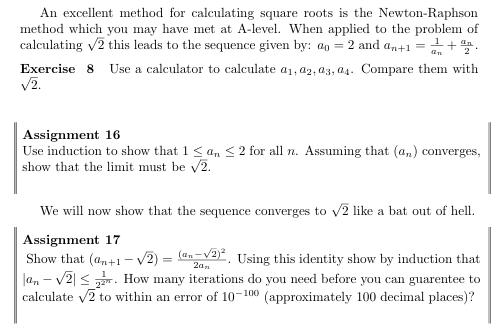
\includegraphics[width=0.8\linewidth]{Term 1/Batoutofhell.jpeg}
    \label{fig:workbook}
\end{figure}

\emph{Quick history lesson: In my year's analysis I module, we had workbooks we had to submit which contained \textbf{over 15 compulsory assignment problems every week!}}

\begin{center}
\huge{\textbf{Permutations}}
\end{center}

Prove that any subgroup of $S_n$ either contains only even permutations, or exactly half the elements are even permutations.

\end{document}